\documentclass{article}
\usepackage[utf8]{inputenc}
\usepackage{amsmath}
\usepackage{graphicx}
\usepackage{hyperref}
\parindent=0pt
\usepackage[a4paper, total={175mm, 252mm}]{geometry}
\usepackage[section]{placeins}
\usepackage{enumitem}
\usepackage{caption}
\usepackage{parskip}

\title{PySpi for Persistent Sources}
\author{Möller, Julius}
\date{May 2023}

\begin{document}

\maketitle


\tableofcontents

\pagebreak


\section{General Procedure}
In contrast to previous approaches to working with INTEGRAL SPI, this method does not attempt to fit the background via physical models, and instead uses a profile likelihood to eliminate its effect in the source model fit. The underlying assumption that allows this to work is that background count rates in each energy bin remain constant for temporally and spatially near SPI Science Windows (SCWs). Here we distinguish between source counts, which describe all detected events directly originating from astronomical objects considered in our source model and background counts, which describe all other detector events.

This works in the following way: once we have split our set of SCWs into clusters within which we claim the assumption of constant background to be true and have defined a source model, a likelihood value can be calculated for each energy bin of each detector in each cluster. If one energy bin of one detector in one SCW with measuring time $t$ has a source count rate $s$ and a background count rate $b$, the probability $P$ of measuring $C$ counts follows a Poisson distribution:
\begin{equation}
    P(C \vert b, s, t) = \frac{\left( t \left( b + s \right) \right) ^C \text{exp}\left( -t \left( b+s\right)\right)}{C!}
\end{equation}

Equivalent energy bins in the same cluster are assumed to have the same background count rate $b$, so that the probability of measuring $C_1$ counts in one SCW and $C_2$ counts in another SCW is simply:

\begin{equation}
    P(C_1, C_2 \vert b, s_1, t_1, s_2, t_2) = P(C_1 \vert b, s_1, t_1) \cdot P(C_2 \vert b, s_2, t_2)
\end{equation}

The likelihood $\mathcal{L}$ for any energy bin of a detector within a cluster depends on all equivalent energy bins in that cluster, i.e. one term for each SCW in the cluster. If we have cluster of size two, the likelihood is described by:

\begin{equation}\label{log likelihood}
    \text{ln}\mathcal{L}(C_1, C_2, t_1, t_2\vert b, s_1 s_2) = \text{ln}P(C_1 \vert b, s_1, t_1) + \text{ln}P(C_2 \vert b, s_2, t_2)
\end{equation}

This expression allows us to solve for the probability distribution of $b$. A full and mathematically correct treatment of the background parameter $b$ turns out to be very cumbersome with only marginal benefits. Hence, the profile likelihood is used by simply solving for the background count rate value $b_M$ which maximizes the likelihood. This is easily done by setting the derivative of equation \ref{log likelihood} to zero and solving for $b$. For a cluster size of two one finds:
\begin{equation}
    b_M = \frac{1}{2} \left[ \frac{C_t}{t_t} - s_t + \sqrt{\left( \frac{C_t}{t_t} - s_t\right)^2 + 4 \left( \frac{C_1s_2+C_2s_1}{t_t}-s_1s_2\right)}\right]
\end{equation}
where $C_t=C_1+C_2$, $s_t=s_1+s_2$, and $t_t=t_1+t_2$. Using this maximum likelihood background $b_M$ finally allows us to compute a likelihood value that is only dependent on the measured counts and the source model:
\begin{equation}
    \text{ln}\mathcal{L}(C_1, C_2, b_M, t_1, t_2 \vert s_1, s_2) = \text{ln}P(C_1 \vert b_M, s_1, t_1) + \text{ln}P(C_2 \vert b_M, s_2, t_2)
\end{equation}
The process for clusters with sizes larger than two is analogous. One such likelihood value exists for every energy bin of every detector in every cluster, such that the total likelihood value for any given source model is simply the sum of the logarithmic likelihoods over all energy bins, detectors, and clusters. Thus the source model may be fitted to the count data by applying an algorithm to maximize the likelihood.

\pagebreak

\section{Spimodfit Procedure}
In order to be able to compare the results obtain using PySpi and the method described above, spimodfit will be used with the same dataset. For the sake of limiting sources of potential errors, the procedure for obtaining results using spimodfit will be described in more detail than might otherwise be deemed necessary. In general, the  \href{https://www-cms.mpe.mpg.de/gamma/instruments/integral/www/}{spimodfit cookbook found here} was followed very closely.

\begin{enumerate}
    \item 
\end{enumerate}


\pagebreak

\section{Results: Crab Nebula}

\begin{figure}[h]
    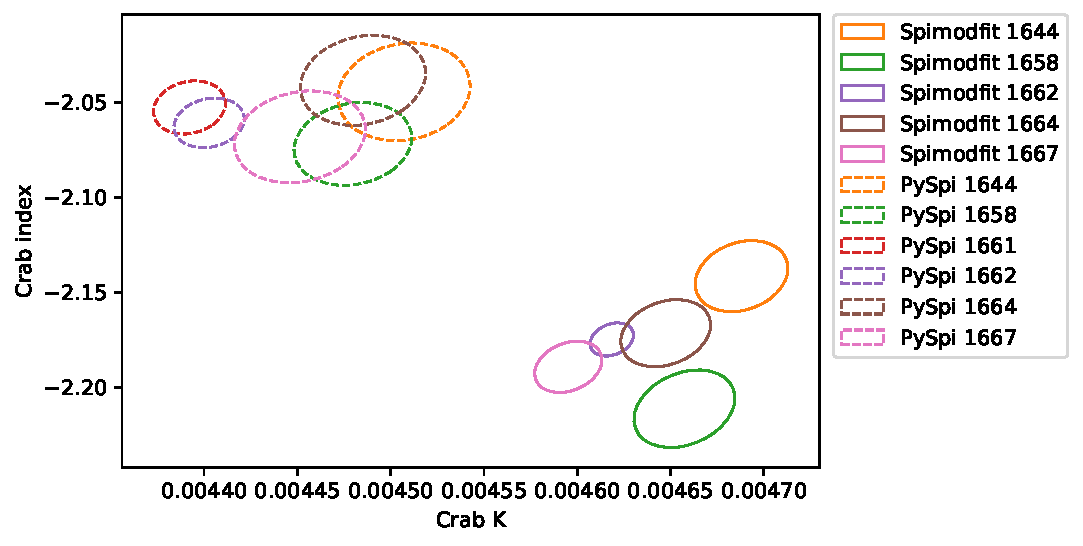
\includegraphics[width=\textwidth]{Images/crab_ps_smf_wo_out.pdf}
    \caption{}
    \label{Crab}
\end{figure}

Figure \ref{Crab} shows one standard deviation confidence intervals of several near SPI Revolutions, as fitted using PySpi and Spimodfit. Revolution 1661 was only fitted using PySpi since spimodfit rejected all SCWs due to "General Expression". The source model is a simple powerlaw 
\begin{equation} \label{powerlaw}
    f(x) = K \frac{x}{piv}^{index}
\end{equation}
where $K$, measured in $\text{keV}^{-1}\text{s}^{-1}\text{cm}^{-2}$ is the differential flux at the pivot value $piv=40$keV, $x$ is the photon energy in keV, and $index$ is the index of the powerlaw.

Both methods used the same energy range of 20-81.5keV, although it is worth pointing out that they use independent algorithms to select which SCWs are used in the fit. PySpi used a cluster size of two. 

Although the two methods obtain different values for the index and normalization, we see comparable sizes of uncertainties as well as similar levels of compactness within the values from different revolutions. 

\section{Results: Simulated Source}
The downside to fitting a real astronomical object such as the Crab nebula is that one can never be exactly sure what the true source parameter values should be. This is why it can be advantageous to simulate a source, feed the simulated data back into the fit, and compare the produced source parameters to the now known true values.

However, not only a simulated source is required, but a background as well. There are different approaches one may take to realize this. The first approach is to use an entirely real dataset from a SPI revolution as background, and add a simulated source on top:

\begin{enumerate}
    \item Choose real data set to use as background. In this case single SPI revolutions were used. For this to work well, there should be as few bright sources within the field of view as possible, since these will interfere with the fit if not included in the source model.
    \item Define spectrum of the source to be simulated, as well as position. In this case powerlaws as shown in equation \ref{powerlaw} are used, and the position of the sources is chosen to be central to as many SCWs in the revolution as possible.
    \item Use the SPI Instrument Response Function (IRF) to calculate the expected source count rates in each energy bin in each detector for each SCW. Multiply by these be the respective lifetime (effectively the active measuring time) of the detector in the SCW, and finally draw a sample of a Poisson distribution with the respective mean to attain the measured counts of the simulated source for each energy bin in each detector in each SCW.
    \item These source count rates are then added to the real measured data we are using as background. 
\end{enumerate}

This dataset can then be used to fit the simulated source with both PySpi and Spimodfit. Although this method of generating the background counts produces a very realistic background, in some cases it may be too realistic by including unwanted sources in the field of view that interfere with the fit. Unlike PySpi, Spimodfit does use a background model, which can also be used in combination with the simulated source:

\begin{enumerate}
    \item When 
\end{enumerate}

\end{document}